\documentclass[border=8pt]{standalone}
\usepackage{tikz}
\definecolor{encre}{HTML}{1B1F2A}
\definecolor{froid}{HTML}{2F5D8C}
\definecolor{brule}{HTML}{C2571A}
\definecolor{repere}{HTML}{8A8F9C}
% Schéma (pas une mesure) : le plan des logits de deux experts, a absent du cache et b résident (le 4e et le 5e du routeur).
% Sans biais, a est choisi si z_a > z_b. Avec le biais beta sur les résidents, a n'est choisi que si z_a > z_b + beta :
% la paroi du polyèdre de décision (z_a = z_b, là où la marge est nulle) glisse d'une largeur beta.
% Les points de la bande étroite changent de choix : a était pris, b l'est maintenant. Le nombre de ces points est la part de cellules changées.
\begin{document}
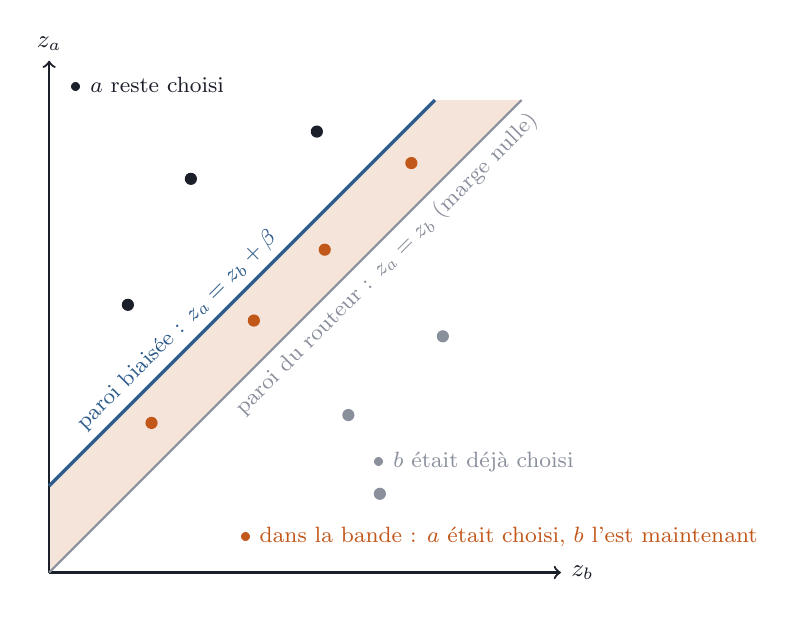
\begin{tikzpicture}[font=\small]
  \def\b{1.1}
  \fill[brule!16] (0,0) -- (6,6) -- (6-\b,6) -- (0,\b) -- cycle;
  \draw[->,encre,thick] (0,0) -- (6.5,0) node[right] {$z_b$};
  \draw[->,encre,thick] (0,0) -- (0,6.5) node[above] {$z_a$};
  \draw[repere,thick] (0,0) -- (6,6);
  \draw[froid,very thick] (0,\b) -- (6-\b,6);
  \node[repere,rotate=45,anchor=north,font=\footnotesize] at (4.1,4.1) {paroi du routeur : $z_a=z_b$ (marge nulle)};
  \node[froid,rotate=45,anchor=south,font=\footnotesize] at (1.8,2.9) {paroi biaisée : $z_a=z_b+\beta$};
  \foreach \x/\y in {1.3/1.9, 2.6/3.2, 3.5/4.1, 4.6/5.2} { \fill[brule] (\x,\y) circle (2.2pt); }
  \foreach \x/\y in {1.0/3.4, 1.8/5.0, 3.4/5.6} { \fill[encre] (\x,\y) circle (2.2pt); }
  \foreach \x/\y in {3.8/2.0, 5.0/3.0, 4.2/1.0} { \fill[repere] (\x,\y) circle (2.2pt); }
  \node[brule,font=\footnotesize,anchor=west,align=left] at (2.3,0.45) {\textbullet\ dans la bande : $a$ était choisi, $b$ l'est maintenant};
  \node[encre,font=\footnotesize,anchor=west] at (0.15,6.2) {\textbullet\ $a$ reste choisi};
  \node[repere,font=\footnotesize,anchor=west] at (4.0,1.4) {\textbullet\ $b$ était déjà choisi};
\end{tikzpicture}
\end{document}
